\chapter{Introduction}

\section{Bioinformatic methods used in genome analysis.}

Bioinformatics is a rapidly developing field of biology and computer science that allows the use of computer algorithms for the analysis and interpretation of large biological data sets. 
Bioinformatic analysis has an increasing value for the pharmaceutical industry as well as for epidemiology \cite{holmes_1995_revealing}.
This interdisciplinary field requires an understanding of many methods of analyzing the data which  put together, provide insight into topics such as the origins of the viruses or their routes of transmission. 
The bioinformatics analysis includes phylogeny, Multiple Sequence Alignment, and Maximum Likelihood Estimation.   


    \subsection{Phylogeny}
Phylogeny is a discipline of science and bioinformatics that refers to the evolution and the origin of the species. 
All of the organisms share a common ancestor, from which all of the species were evolving through a mechanism of natural selection.
Due to random mutations, an organism either gains or loses a trait that may be beneficial for its survival. 
The relationship and ancestry of the species can be studied through phylogenetic analysis and the construction of phylogenetic trees, which are a visual representation of the relativeness of the organisms.  
Phylogenetic analysis has an important application in virology and epidemiology where it is used to construct transmission models or to determine the origin of the transmission of viruses.
A typical phylogenetic tree structure consists of the root, which represents the ancestor organism, and the branches that stem from it. 
Another feature of the phylogenetic trees is the external and internal nodes. 
An external node is a representation of the virus that was sequenced and analyzed, whereas the internal nodes are the supposed ancestor viruses of the ones that were sequenced.
Some of the branches are referred to as clades, which represent all the descendant sequences from one ancestor (Pevsner, 2015). 

    \subsection{Multiple Sequence Alignment}

To produce a phylogenetic tree the sequences need to be obtained from one of the many databases available online which specialize in the virus or organism of interest. An example of such a database can be the Los Alamos database which stores millions of HIV sequences. 
The sequences stored in those databases are submitted with respect to the anonymity of the infected patients and are referred to by their accession codes. 
Once the sequences are obtained they need to be aligned.
There are two methods of aligning the sequences which depend on the number of sequences that need to be analyzed. 
Pairwise alignment is used for two sequences, for three and more sequences the algorithm used is referred to as Multiple Sequence Alignment. 
There are many approaches to this method one of them being ClustalW which is considered a progressive alignment. 
This approach was used mostly in the past and was the most widely used from the 1990s.
Currently, faster and more efficient approaches to Multiple Sequence Alignment are recommended.
One of them is MUSCLE, which together with PRALINE and InterAlign is considered to be an iterative approach \cite{pevsner_2015_bioinformatics}. 
Both ClustalW and MUSCLE approaches are available as a setting in the program MEGA11 (Molecular Evolutionary Genetics Analysis) which offers sequence alignment as well as phylogenetic analysis of the sequences.

        \subsubsection{FigTree}

Analyzed sequences can be evaluated through qualitative analysis. 
A very useful program that provides a good visual representation of the phylogenetic tree is Figtree, which allows editing of the tree branch colors and highlighting tools that make the tree easier to look at. 
The countries from which the sequence was obtained can be color-coded, i. e. the branches from one country are all colored in one specific color.
Coloring the branches of the tree is a great method that helps find some interesting clades within the tree faster than normal. 

        \subsubsection{Bootstrapping} 

A qualitative analysis alone is not considered a proper investigation of the sequences, and statistical tests need to be performed to determine the factual state of the sequence relativeness. 
A method that is frequently used in statistics, bootstrapping, has its application in phylogenetic analysis as well. 
In statistics, bootstrapping involves many series of data re-sampling in order to test a hypothesis.
In bioinformatics, bootstrapping offers a quantitative analysis of the sequences by testing, how certain it is that the branch or a clade re-assorts itself in the same way \cite{ojha_2022_computational}
The bootstrap values are represented in the range between 0-100. The higher the value, the more probable it is that the sequences are correctly positioned within a phylogenetic tree. 
In bootstrap analysis, any value that exceeds 70 is considered statistically relevant, and the sequences which obtained such values are considered to be related with high probability. 

\section{Human Immunodeficiency Virus (HIV).}

World Health Organisation (WHO) has stated that approximately 38.4 million people were struggling with HIV infections. 
People who are at risk of contracting the virus are sexually active homosexual men and PWID (Persons Who Inject Drugs), however, any person can get infected with the virus through sexual activity or the use of un-sterile sharp objects).\cite{worldhealthorganization_2021_hivaids}\\
HIV belongs to the genus \textit{Lentivirus}, and similarly, as the other viruses belonging to this genus, HIV shows a long incubation period.
This trait of HIV complicates the process of diagnosis.
Another example of the virus from this genus is Simian Immunodeficiency Virus (SIV) which is closely related to HIV.\\
Further classification of the virus places it in the \textit{Retroviridae} family.
Viruses belonging to this family, HIV included, can initiate the use of reverse transcriptase which allows it to reverse the transcription process and convert their RNA to double-stranded DNA. This allows the virus to integrate with the human DNA using the enzyme integrase. \cite{fanalesbelasio_2010_hiv} \\
HIV infects the immune cells, CD4+ T-lymphocytes. 
Once the cell is infected, the virus uses the reverse transcriptase enzyme to convert its RNA genome into DNA, which is later integrated with the cell's own DNA. 
This process allows the virus to become latent.
In this state, the transcription of the viral genome is very low, and as a result, the infected cell is not targeted by the T-cell-mediated cytotoxicity. 
This provides an effective reservoir for HIV infection. \cite{chen_2022_the}
Gracia et. al states that this stable reservoir of HIV within the resting-memory CD4+ T-cells is currently the main issue with eradicating HIV. \cite{garca_2020_transcriptional}\\
An important role in the natural response to HIV is played by CD8+ cytotoxic T-lymphocytes which can use the MHC Class I (Major Histocompatibility Complex) molecules on their cell surface to detect HIV-infected CD4+ helper T-lymphocytes. 
An infected cell can be then destroyed by the activation of the infected cell’s death receptors by the death-inducing ligands on the surface of cytotoxic T-cells. \cite{gulzar_2004_cd8}
However, as stated by Collins this mechanism is not effective enough to eradicate the virus once an individual was infected. \cite{collins_2004_resistance}
Due to this reason, patients infected with HIV rely heavily on the combination of various anti-viral drugs. \cite{worldhealthorganization_2021_hivaids}

    \subsubsection{Structure and Genome}

Figure 2.1 represents the diagram of the HIV genome. 
The entire RNA strand is equal to approximately 9.7 kilobase pairs.


\begin{figure}[h]
  \centering
  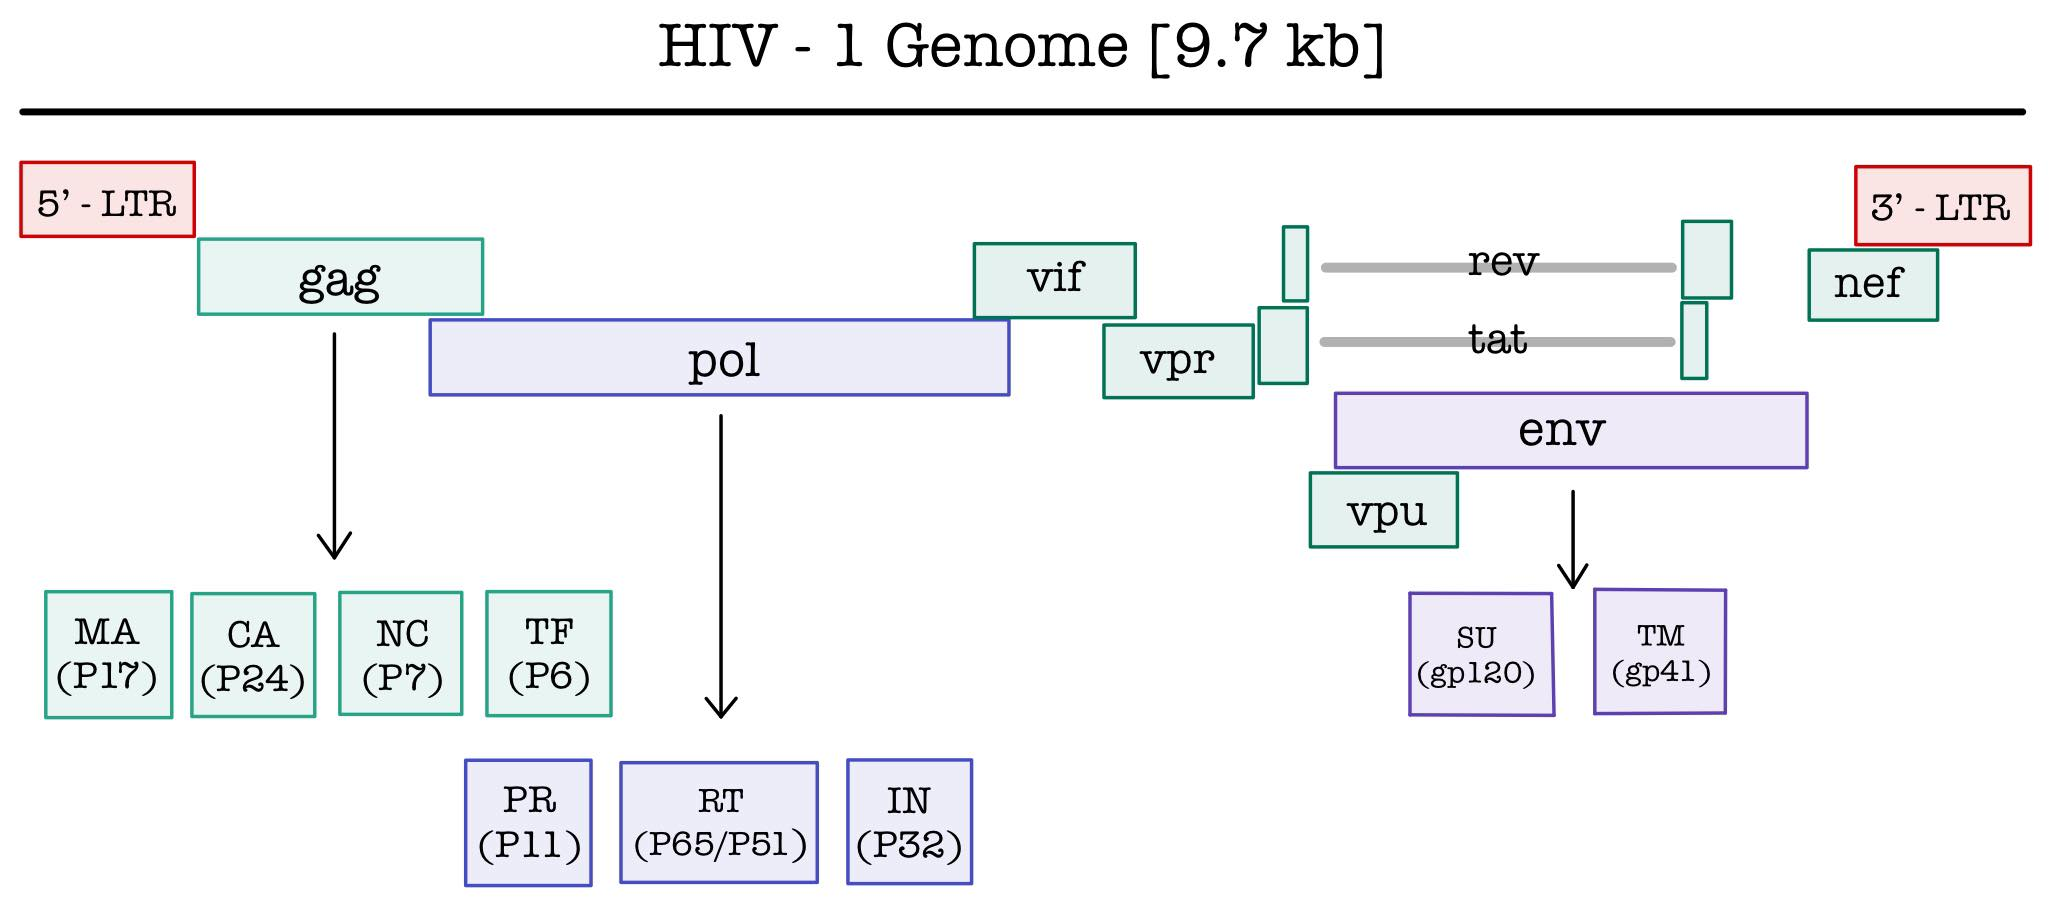
\includegraphics[width=0.85\textwidth]{images/hiv genome.jpg}
  \caption{A diagram representing the structure of the HIV-1 genome. \textbf{Red:} LTR sequences flanking the genome. \textbf{Bright Green:} \textit{gag} gene including MA - outer membrane, CA - capsid; NC - nucleocapsid. \textbf{Blue:}
  \textit{pol} gene including PR - protease gene, RT - reverse transcriptase gene, IN - integrase gene. \textbf{Purple:}:
  \textit{env} gene including SU - gp120 surface protein and TM - gp41 trans-membrane protein. \textbf{Dark Green:}: regulatory proteins.}
  \label{fig: HIV -1 genome}
\end{figure}

According to Seitz, the genome structure is flanked by the LTR sequence which acts as the promotor at the 5' end. 
Further down the sequence follows \textit{gag} gene which contains sequences for the outer membrane, capsid protein, nucleocapsid, and stabilizing proteins. 
Next in the genome is \textit{pol} gene, which encodes the genes for various enzymes useful for the virus including protease, which was the target region of the sequences used during this project. 
Other enzymes encoded within the \textit{pol} gene include the reverse transcriptase mentioned above, and integrase (which allows HIV to integrate its genome with human DNA. 
The last significant gene within the HIV genome is \textit{env} gene which encodes for surface proteins (gp120 and gp41).\cite{seitz_2016_human}\\
The remaining sequences code for the accessory proteins which have their individual functions. 
The first accessory protein from the 3’ direction is \textit{nef}, which main role in sustaining a high level of viral replication. 
The next accessory sequence is \textit{}{rev} is responsible for the regulation of protein expression, followed by the \textit{tat} which binds to the TAR hairpin at the 5’ end of the new RNA, enhancing the transcription.\cite{turner_1999_structural}\\
From the 5’ direction of the HIV genome, \textit{pol} sequence is followed by another accessory protein sequence \textit{vif}.
Zhang et. al. suggested that this protein could be responsible for the folding of the viral RNA.\cite{zhang_2000_human}
The next accessory protein in the genome is \textit{vpr} which is responsible for transporting the pre-integration complex into the host cell’s nucleus. \cite{kogan_2011_hiv1} 
The last accessory protein is \textit{vpu} which is responsible for the CD4+ proteins destruction and enhances the process of virion release from the cell. \cite{khan_2021_role}

        \subsubsection{HIV - Origins of transmission}

The first transmission of HIV from chimpanzees to humans was estimated by Eberla and Guertler to be around the 1930s with a standard 
deviation of 20 years.\cite{eberle_2012_hiv}
\textit{P. troglodytes troglodytes} were predicted to be the source of the ancestor of many HIV viruses circulating around the world.


        \subsubsection{HIV1 - B}

Figure 2.2 depicts the distribution of HIV-1 subtype B infections around the world.\\
HIV has two main types. 
Type 1, which is recognized as the pandemic causing, is responsible for over 90 percent of infections. 
HIV-1 has 4 recognized groups of the virus - M, N, O, and P.
The most predominant group within HIV–1 (M) is responsible for over 99.6 percent of infections within this group.\cite{kandathil_2005_molecular}
Sub-type B, which is the core subject of this project, also belongs to this group. 
According to  Holmes et. al., this sub-type is responsible for infections in the developed world (Europe, North, and South America). 
Other subtypes, such as C, are most predominantly found in Central and West Africa. \cite{holmes_1995_revealing}
According to Paraskevis et. al., Sub-type B of HIV-1 originated in the United States from a single mutation from Haiti in the late 1960s. 
Since then, this sub-type was transmitted effectively into Western Europe and become the predominant sub-type in this region. 
The Eastern part of Europe was not introduced to this subtype until the migration between the West and the East of Europe became more accessible.\cite{paraskevis_2009_tracing}

\begin{figure}[h]
  \centering
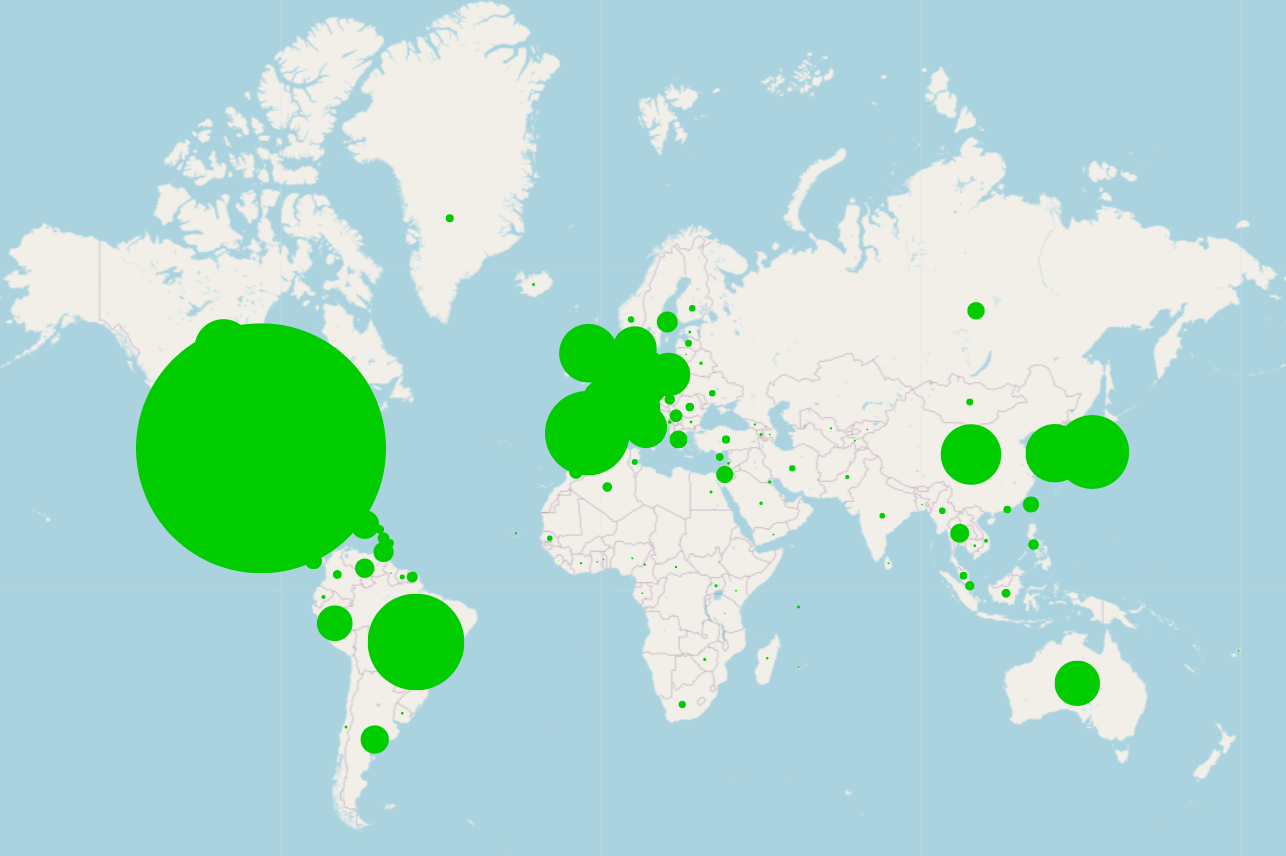
\includegraphics[width=0.6\textwidth]{images/HIV1B spread across the world.png}
  \caption{Distribution of the HIV - 1 subtype B infection around the world. The size of the circle indicates the number of sequences uploaded to the Los Alamos database per country. The picture was generated on the database website.} %
  \label{fig: HIV-1 B around the world.}
\end{figure}

\section{Aims and Objectives}
The aim of this research was to evaluate the bioinformatic analysis methods such as phylogeny, multiple sequence alignment, and bootstrap analysis,  as a tool for tracing the spread and evolution of the viruses based on the transmission model of the HIV – 1 subtype B within Eastern Europe.
    \subsubsection{Hypothesis}

    Based on the review of the available literature regarding the transmission and the geopolitical situation it could be hypothesized that HIV-1 subtype B transmission events in Eastern Europe happen between countries that share a common history more frequently compared to countries that are just geographically near each other. 